% !TEX TS-program = xelatex
% !TEX encoding = UTF-8
% !Mode:: "TeX:UTF-8"

\documentclass[onecolumn, oneside, ctexart]{SUSTechHomework}
\setlength{\parindent}{2em}
\linespread{1.5}

\coursecode{CS305}
\coursename{Computer Networking}
\title{PAssignment 2}
\date{Apr. 24, 2022}

\begin{document}
\maketitle



\section{Design of System}

\subsection{HTTP}

\paragraph{Environment} This program was written under \emph{Python 3.8}, exclude the buildin packages, it also uses asyncio 3.4.3 and flask 2.1.1. Since everyone should has asyncio, you may only check or install flask via
\begin{minted}{shell}
pip install Flask
\end{minted}

I threw away the skeleton provided, and use \emph{Flask} to provide the basic operations needed by designing a REST api. The server provides five endpoints:
\begin{minted}{python}
@app.route('/', methods=['GET'])
def get_page():
    pass
    
@app.route('/vs/<vid>', methods=['GET'])
def get_video_part(vid):
    pass
    
@app.route('/danmaku/<vid>', methods=['GET'])
def get_danmakus(vid):
    pass
    
@app.route('/chat/<vid>', methods=['GET'])
def get_chat_history(vid):
    pass
    
@app.route('/danmaku/<vid>', methods=['POST'])
def post_danmaku(vid):
    pass
\end{minted}

\par As mentioned in the document, the requests sent to route "/" (aka. http://localhost:8765/) will get a response, whose body is \textit{danmu.html}, with two params filled by render\_template (including the url for the background, and the client id assigned by the server).
\par The danmakus service uses "/danmaku" endpoint. Since we have multiple videos, we need to store the danmakus for different video separately, thus we put the video id into the url, other constraints are placed into parameters, as the REST style. All \emph{POST} requests are handled by \emph{post\_danmaku} function, and the \emph{GET} requests are handled by \emph{get\_danmakus} function.
\par Since I implemented the down streaming for the video, the \emph{get\_video\_part} listening GET requests to "/vs". Each response contains part of the video file, and the video component in html5 will auto request the next part of file until EOF. Also, hope you enjoy the three fantastic Apple ads selected as the resource :)
\par Different from the danmakus show flowing above the video, which uses the relative time of a danmaku was sent in a video as the filter, the chat board displaying in the right side cares more about the absolute time of one danmaku was sent.\\

\centerline{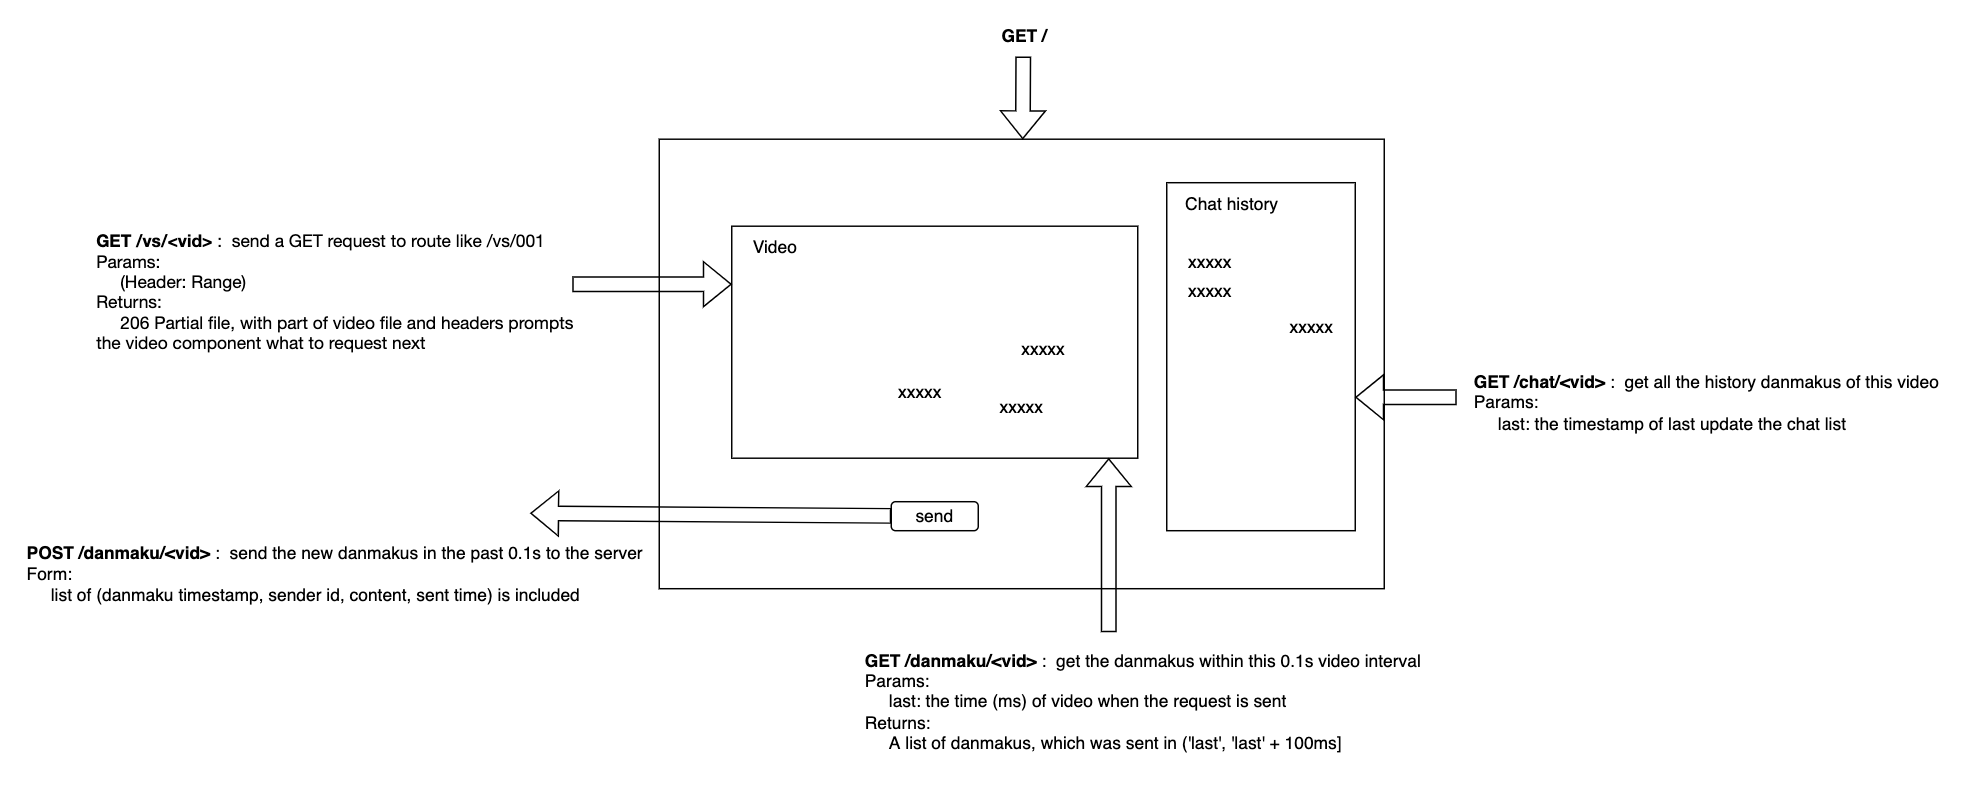
\includegraphics[width=\textwidth]{res/http}}

\par Note that for the bonus part, the live mode is integrated into the video mode, since the document mentioned "don't need to focus on the live contents", I use the videos as live, aka display a chat board that display the talking person nearly real-time (with some polling delay).\\

\centerline{\includegraphics[width=0.7\textwidth]{res/intro}}


\subsection{WebSocket}
Rather than the HTTP version, WebSocket is quiet easy, and the provided skeleton is good enough to implement the danmakus. Since this protocol is \emph{full duplex}, the server can not only receive messages from clients (of course), but also send message to client, or broadcast message to clients.
\par As the comments in the code said, the \emph{websockets.serve} listens and handles connections to localhost:8765. When a new client is connected (after opening the html file in the browser, the js command \textit{let ws = new WebSocket('ws://localhost:8765')} will create a new client socket and connect to the server socket), a new async function reply will be called and keep running in background, until a ConnectionClosed is raised to stop this thread.
\par Assume that there are $n$ websites opening (normally they should keep connecting with the server), they are considered as $n$ client sockets and all added into the clients list of a DanmakuServer instance. In all the time, there are $n+1$ threads, one holds the main, and other $n$ threads each contains a reply. In the most of time, the function is blocked by the async for, once a client sends message to the server, the corresponding thread's function will step into a for loop, in which the server broadcast the message to the list of clients.


\section{Running Results}

\subsection{HTTP}
Since the logic seems correct for me, the HTTP version can support infinite users theoretically, and the display of danmakus has no missing or repeat, and low latency. However, since we have to use polling for HTTP, which will cause a lot of CPU and memory cost, I've tested opening 8 webpages at one time and the fan began running fast.

\par The \emph{video mode} shows danmakus not in real time, but bases on the time of video, as shown below. But you may also notice that the chat board floating in the right side of webpage shows danmakus in the realtime, base on the time it was sent, but not about the time in the video, that's for the \emph{live mode.}\\

\centerline{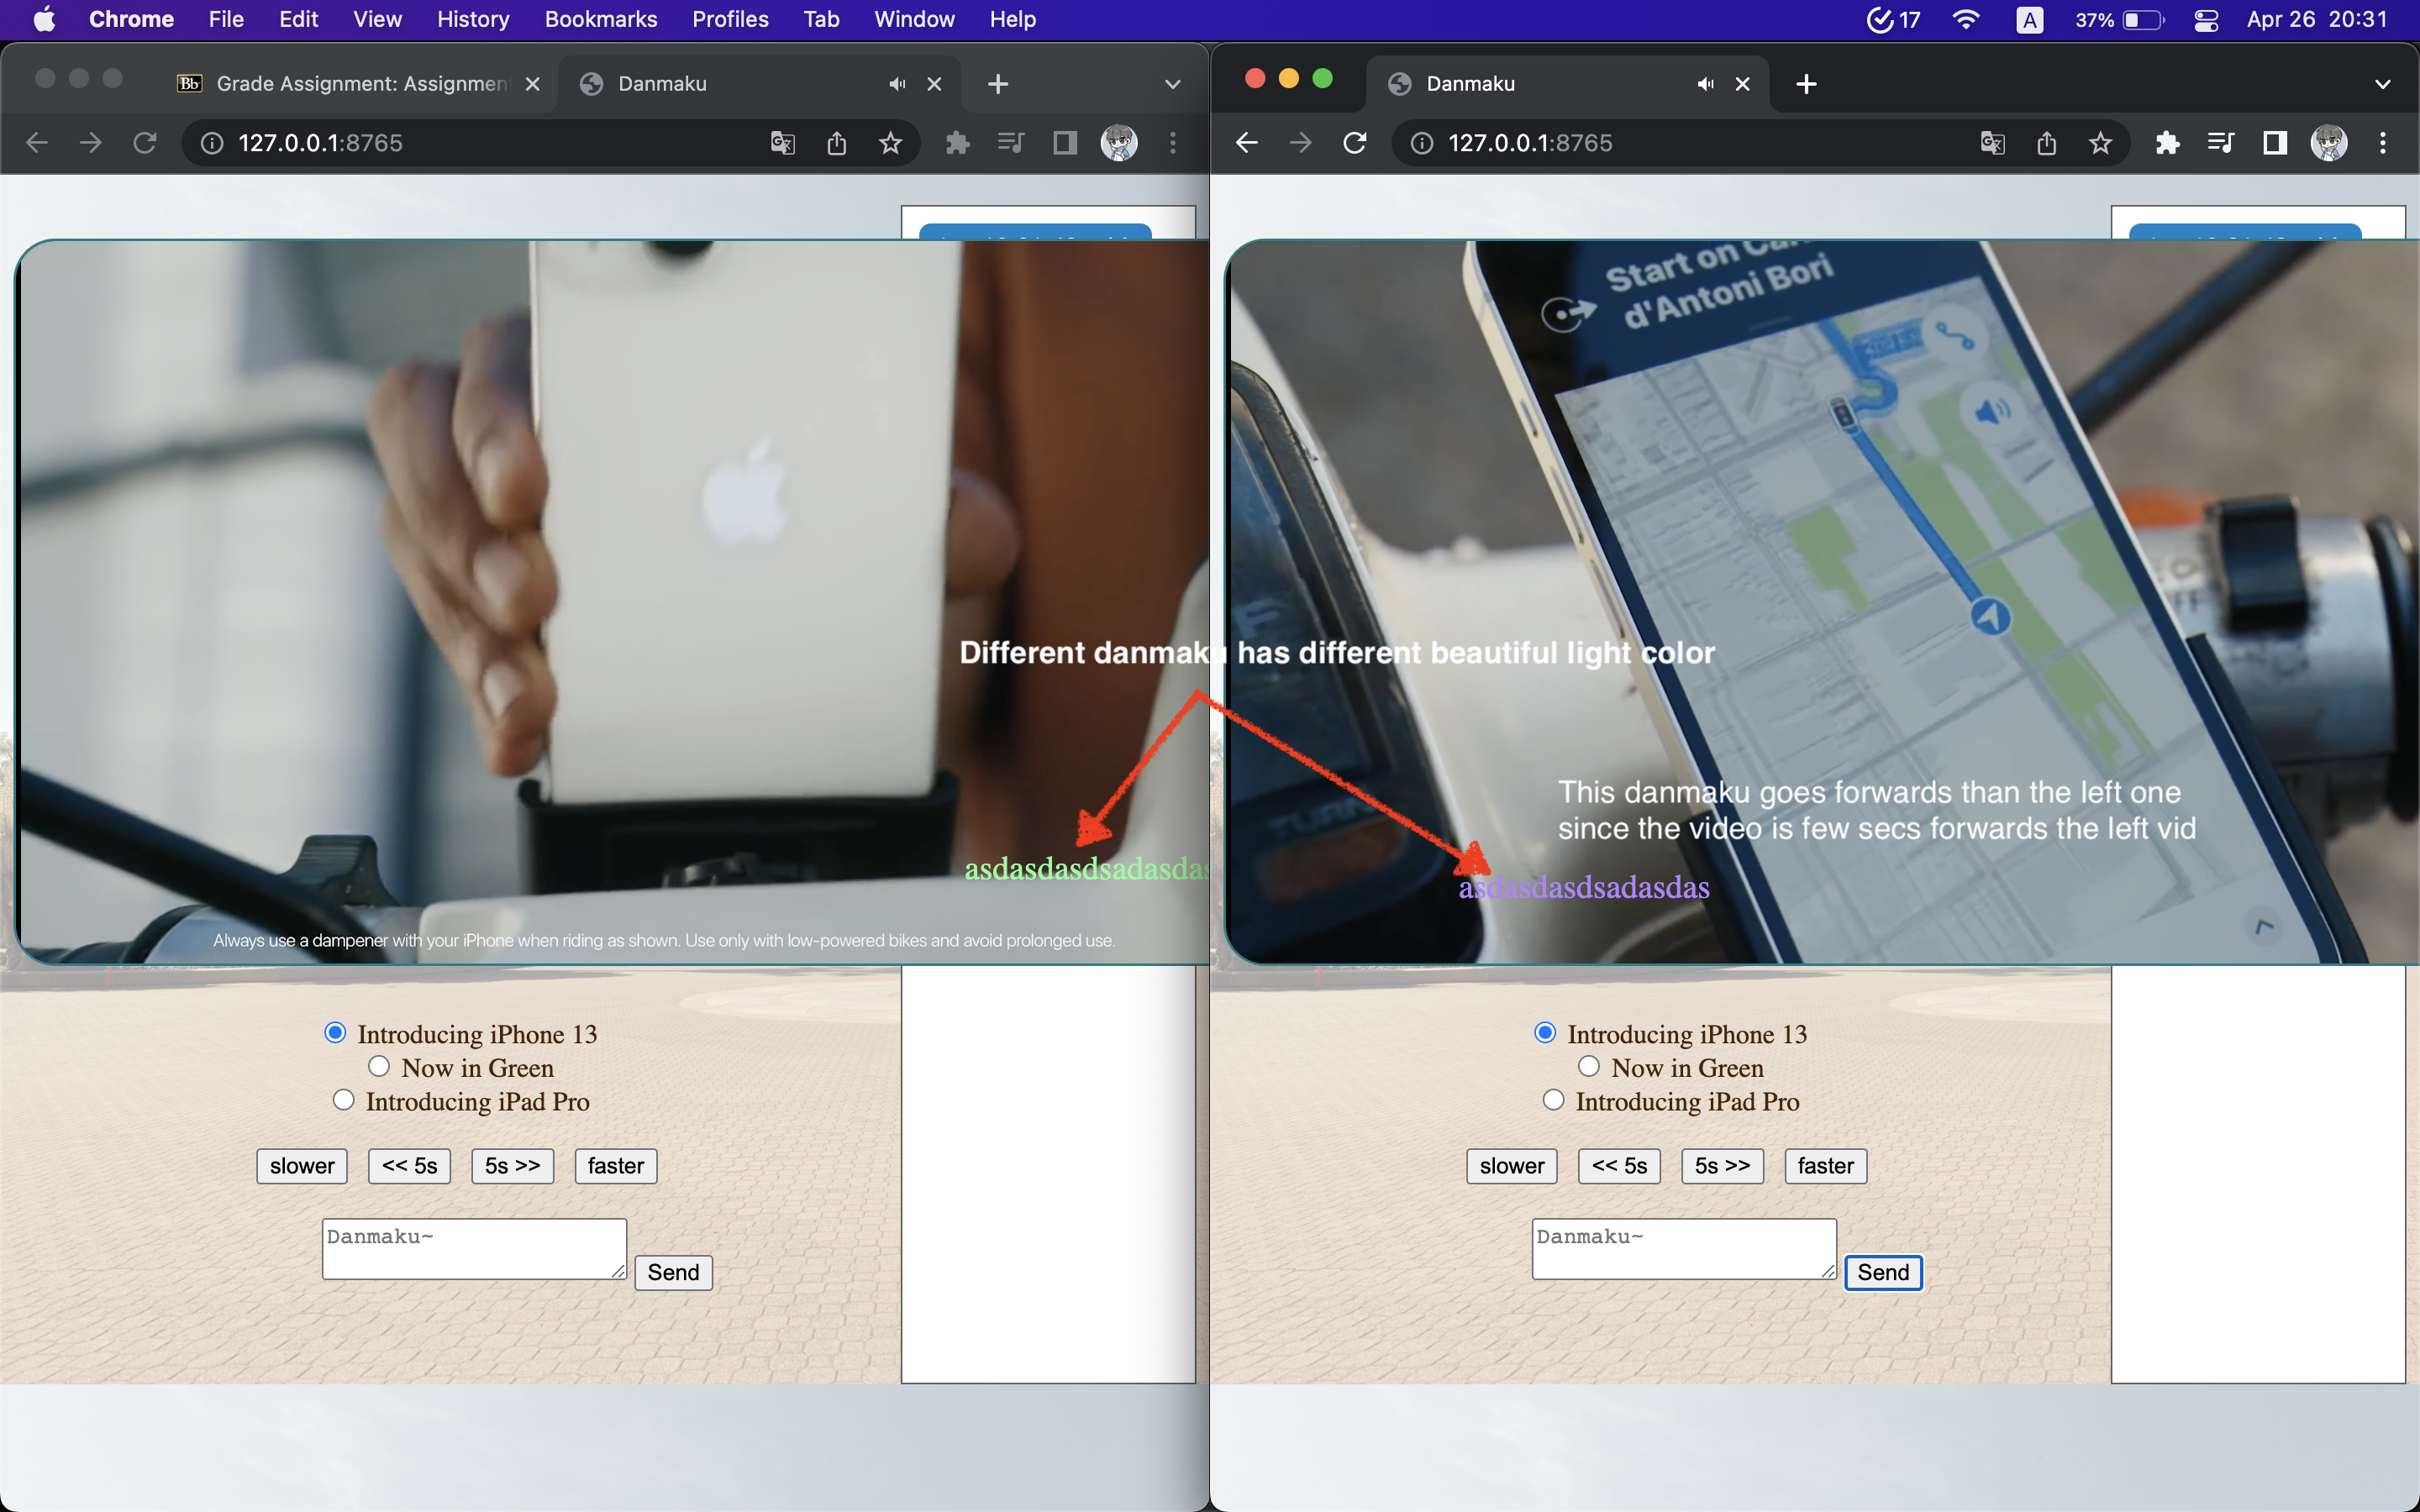
\includegraphics[width=0.6\textwidth]{res/vid-mode}}

\noindent
* The page has been beautified, such as adding a background picture, and changing the color of danmakus.\\
** Please use Chrome if the video component looks strange or cannot click play/pause in other browsers.

\par Packages can be caught by Wireshark (Loopback: lo0, set the display filter as tcp.port == 8765) or F12 Network watcher.\\

\centerline{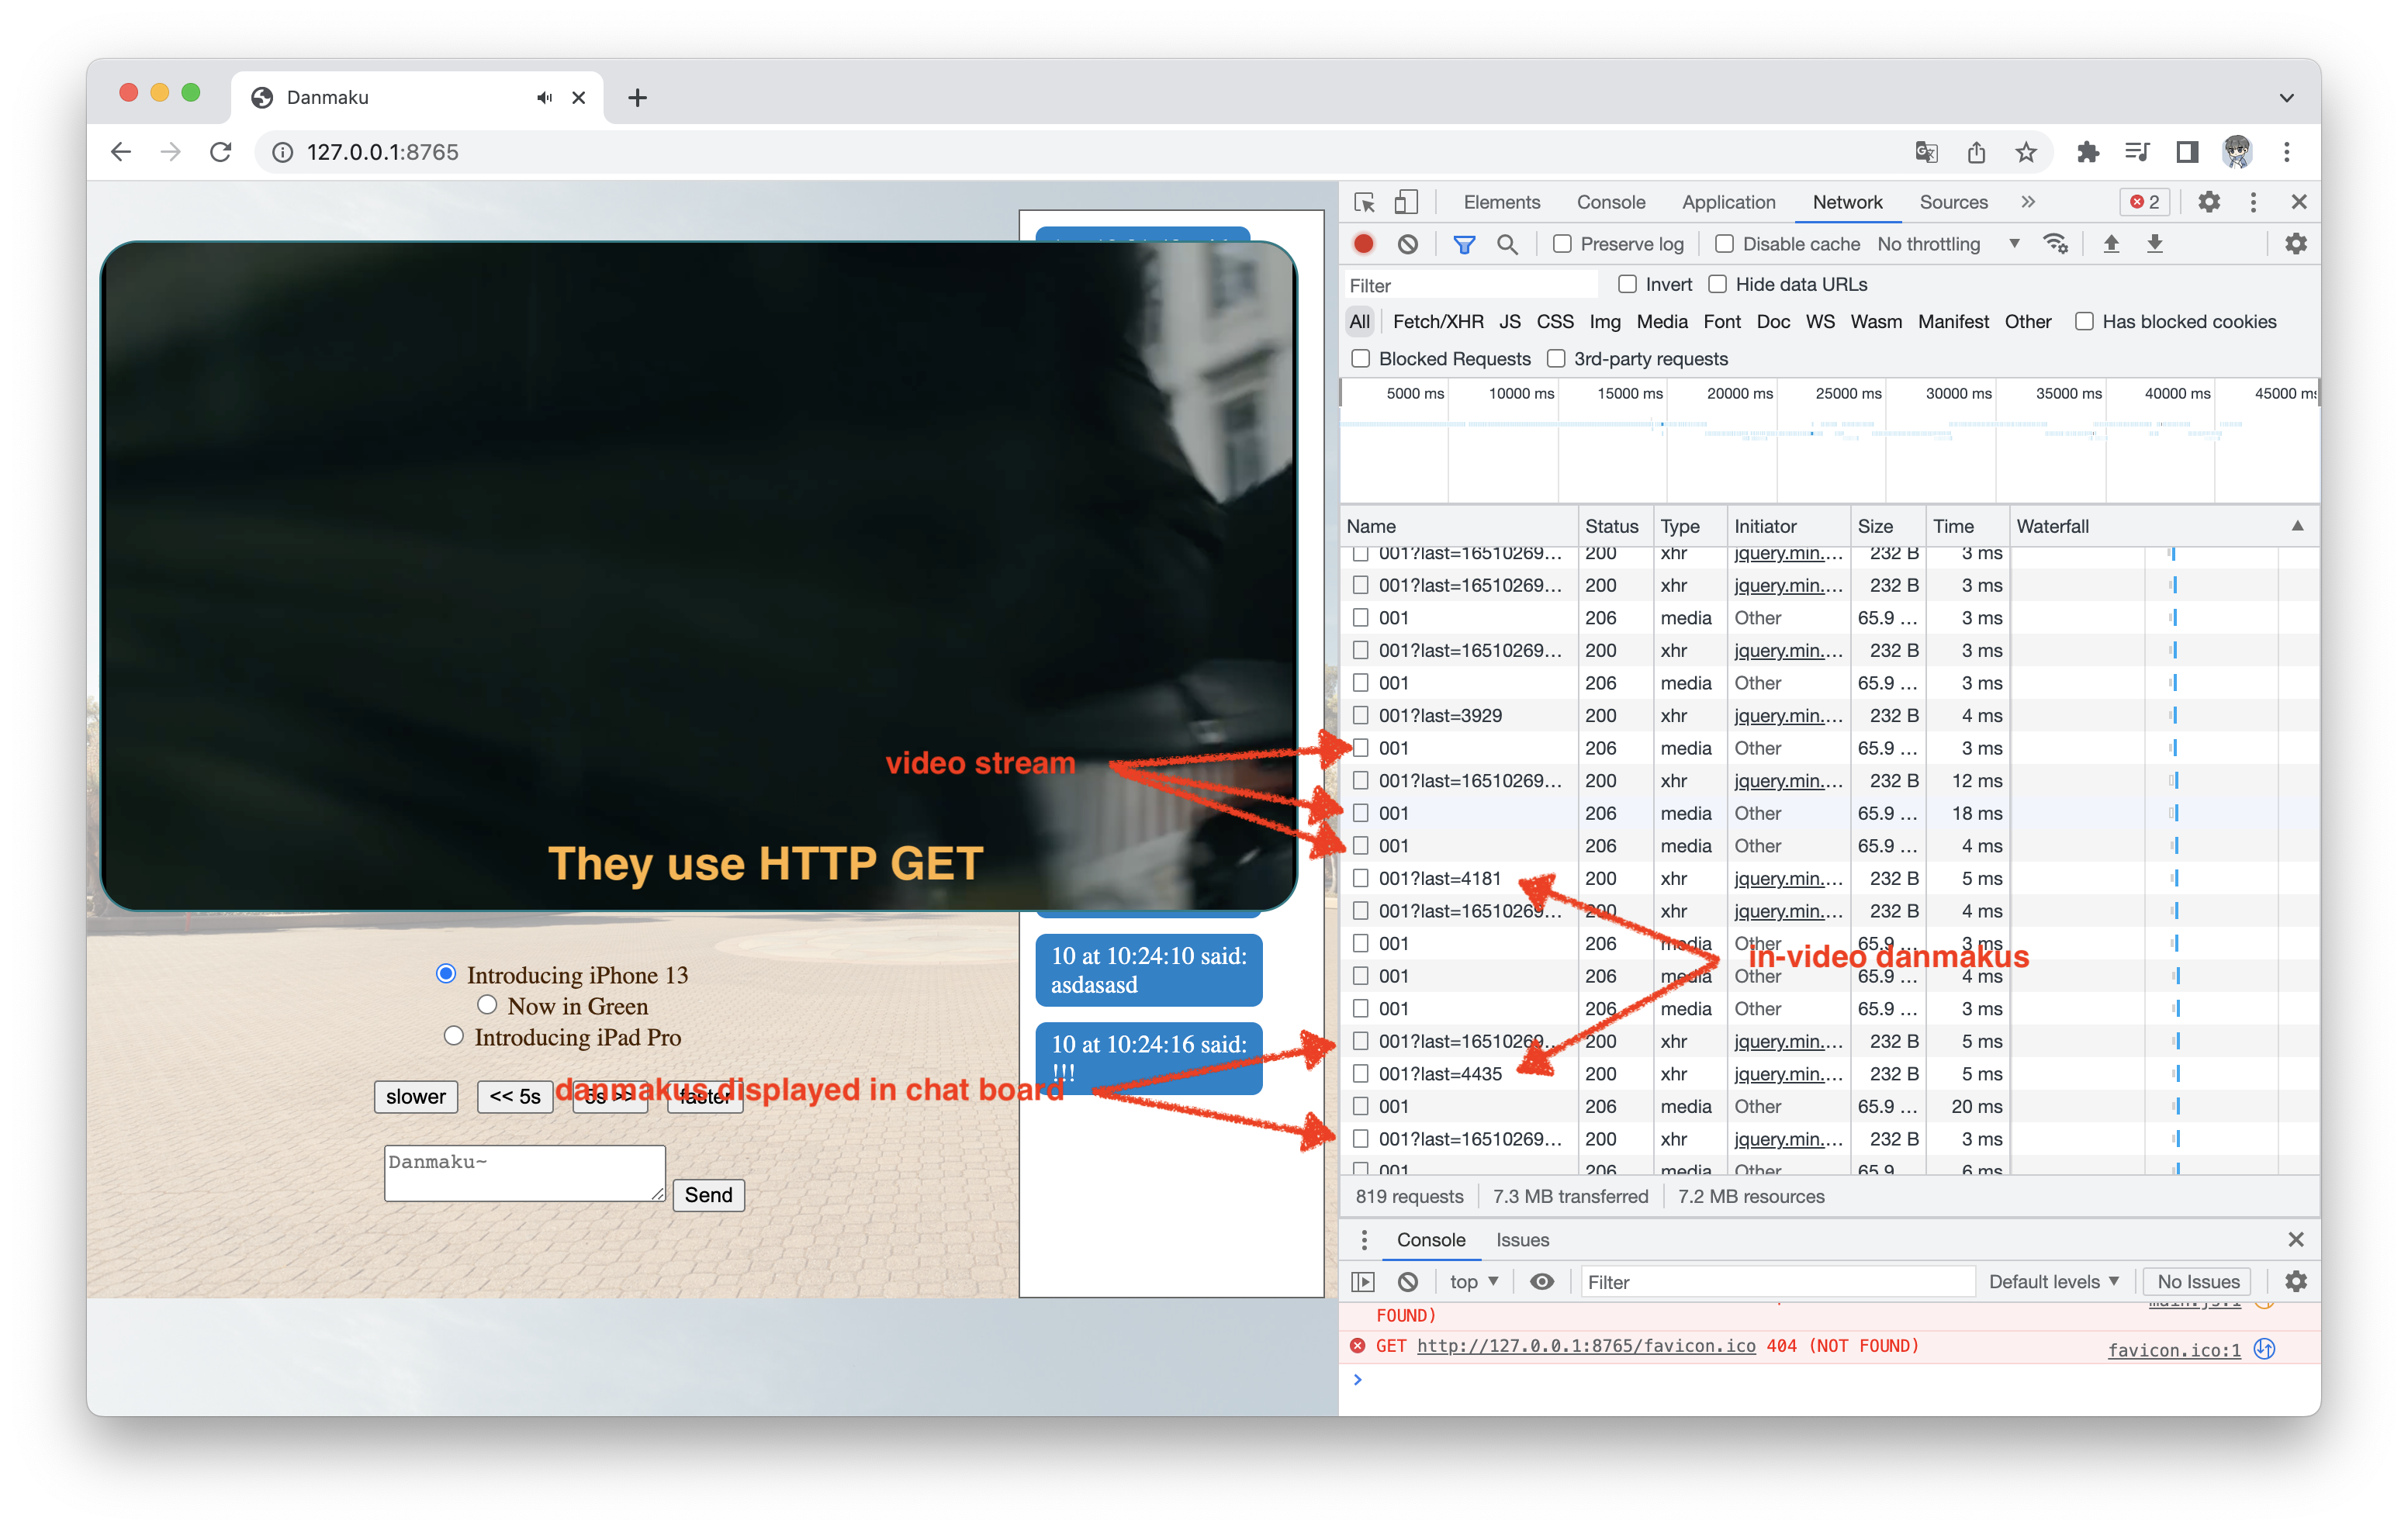
\includegraphics[height=14em]{res/http0}\quad
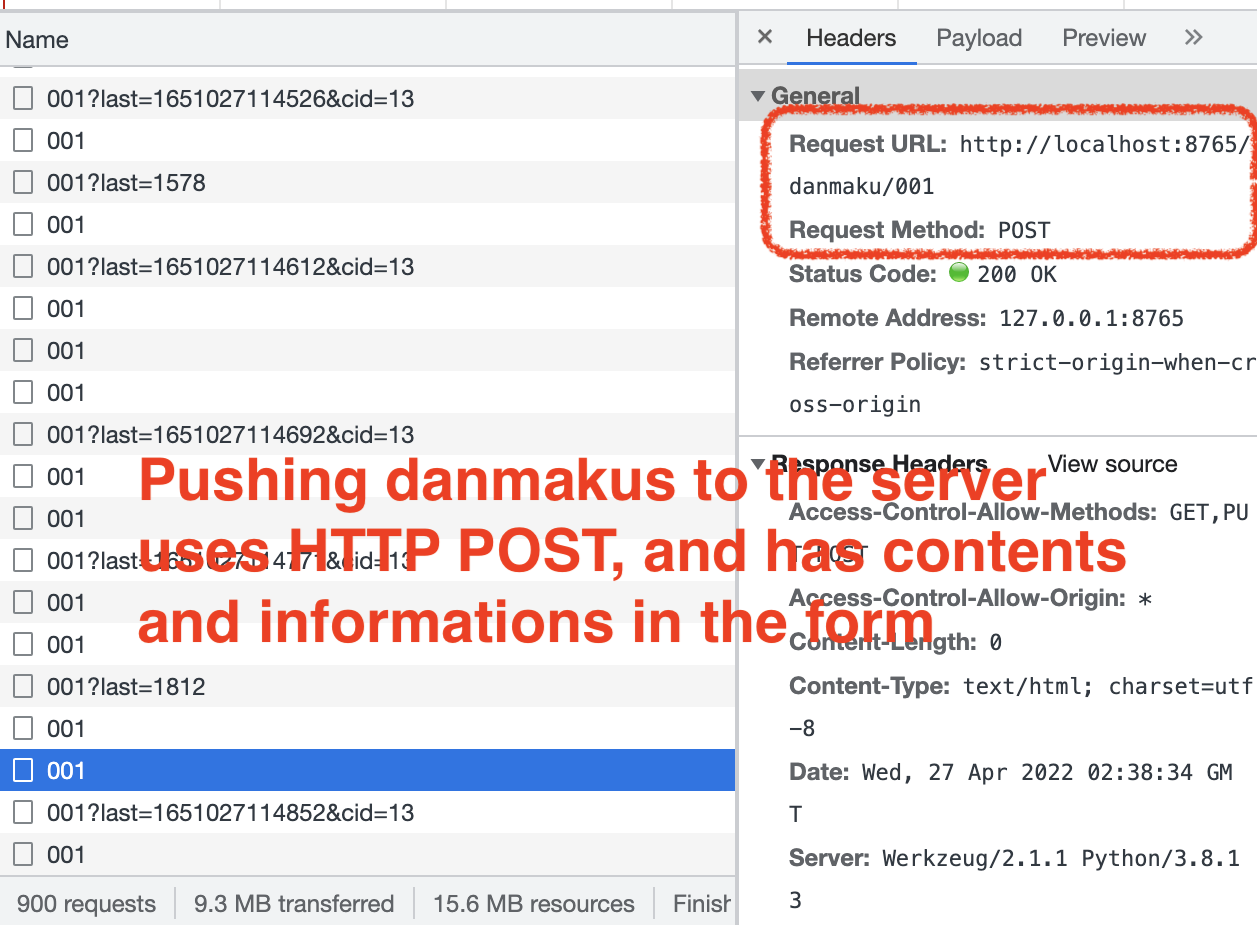
\includegraphics[height=14em]{res/http1}}

\section{WebSocket}
The ws version is just the baseline, without any additional method. As below shows, opening many clients in the same time has the correct effect as we expected. Moreover, since ws is full duplex, we need no stupid and CPU/memory/IO costing pollings. We can easily open 10+ webpages without adding much workload.\\

\centerline{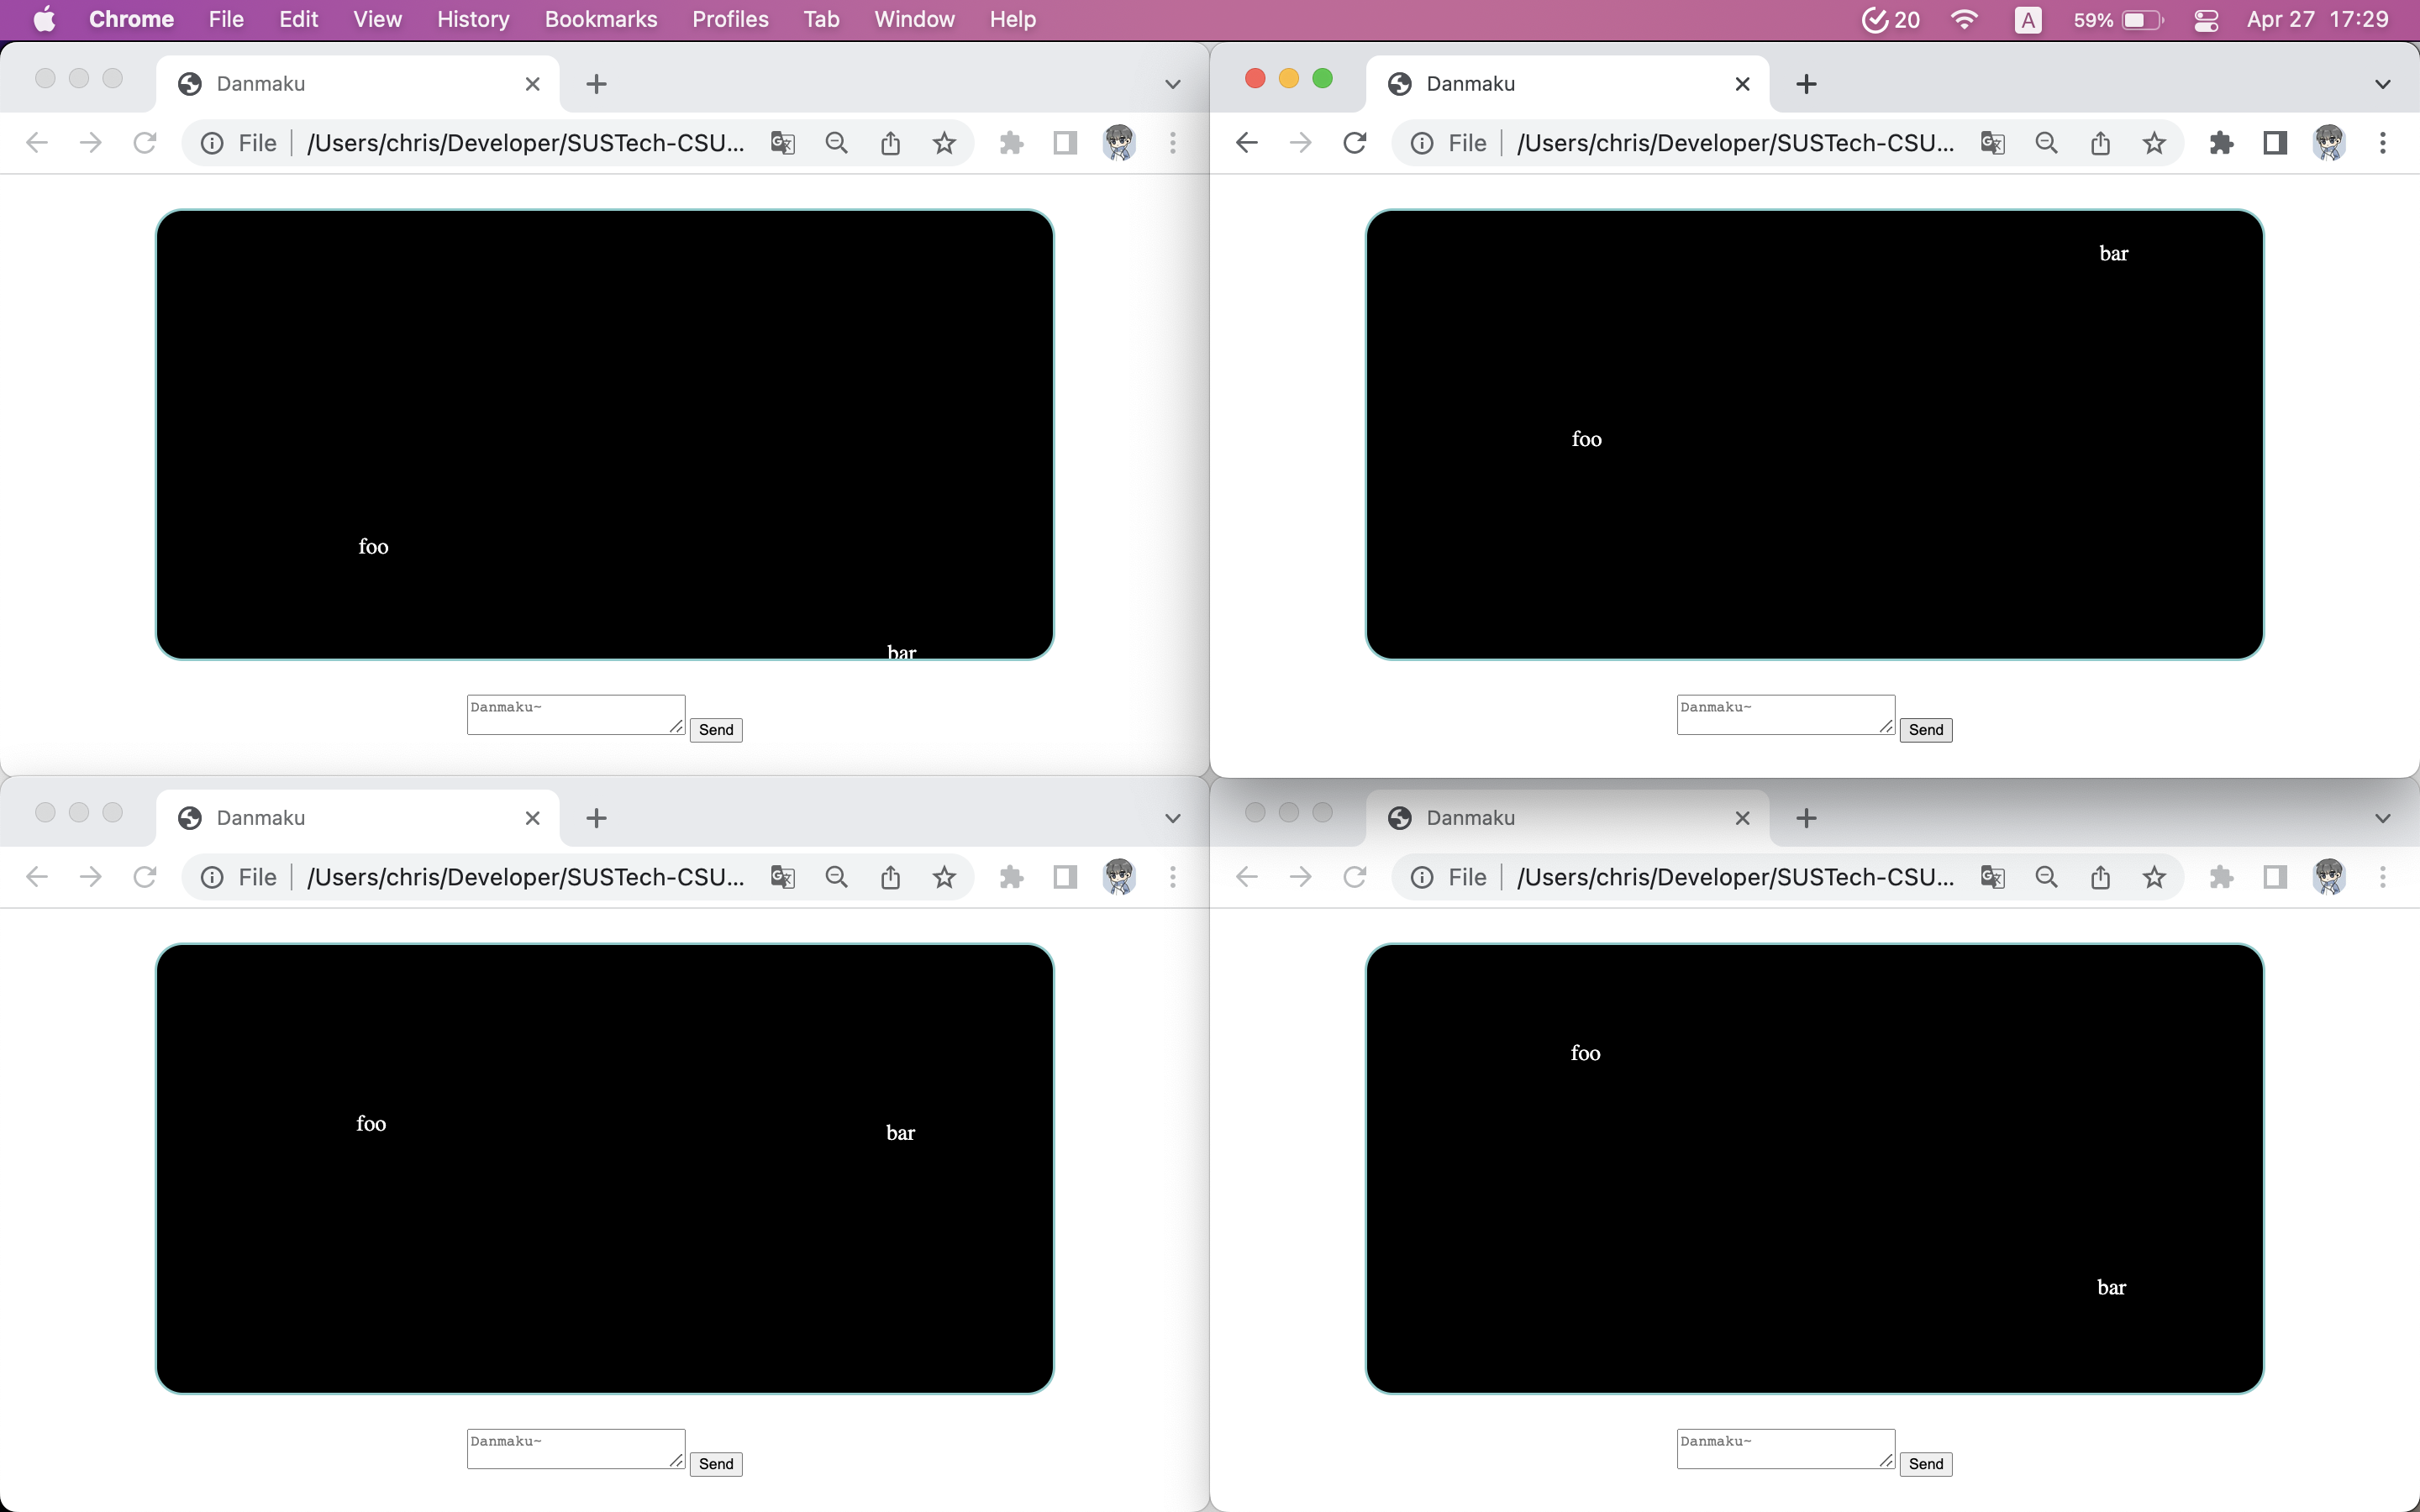
\includegraphics[width=0.6\textwidth]{res/wss}}

\par Chrome's developer tool doesn't support capture packages under WebSocket protocol, as below shows. But we can capture the packages by using Wireshark, setting the display filter as \emph{websocket}.\\

\centerline{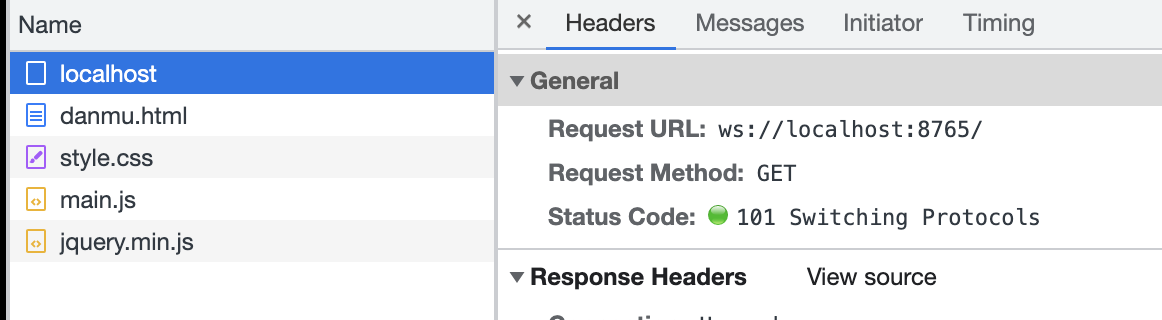
\includegraphics[height=6em]{res/wsc}\quad
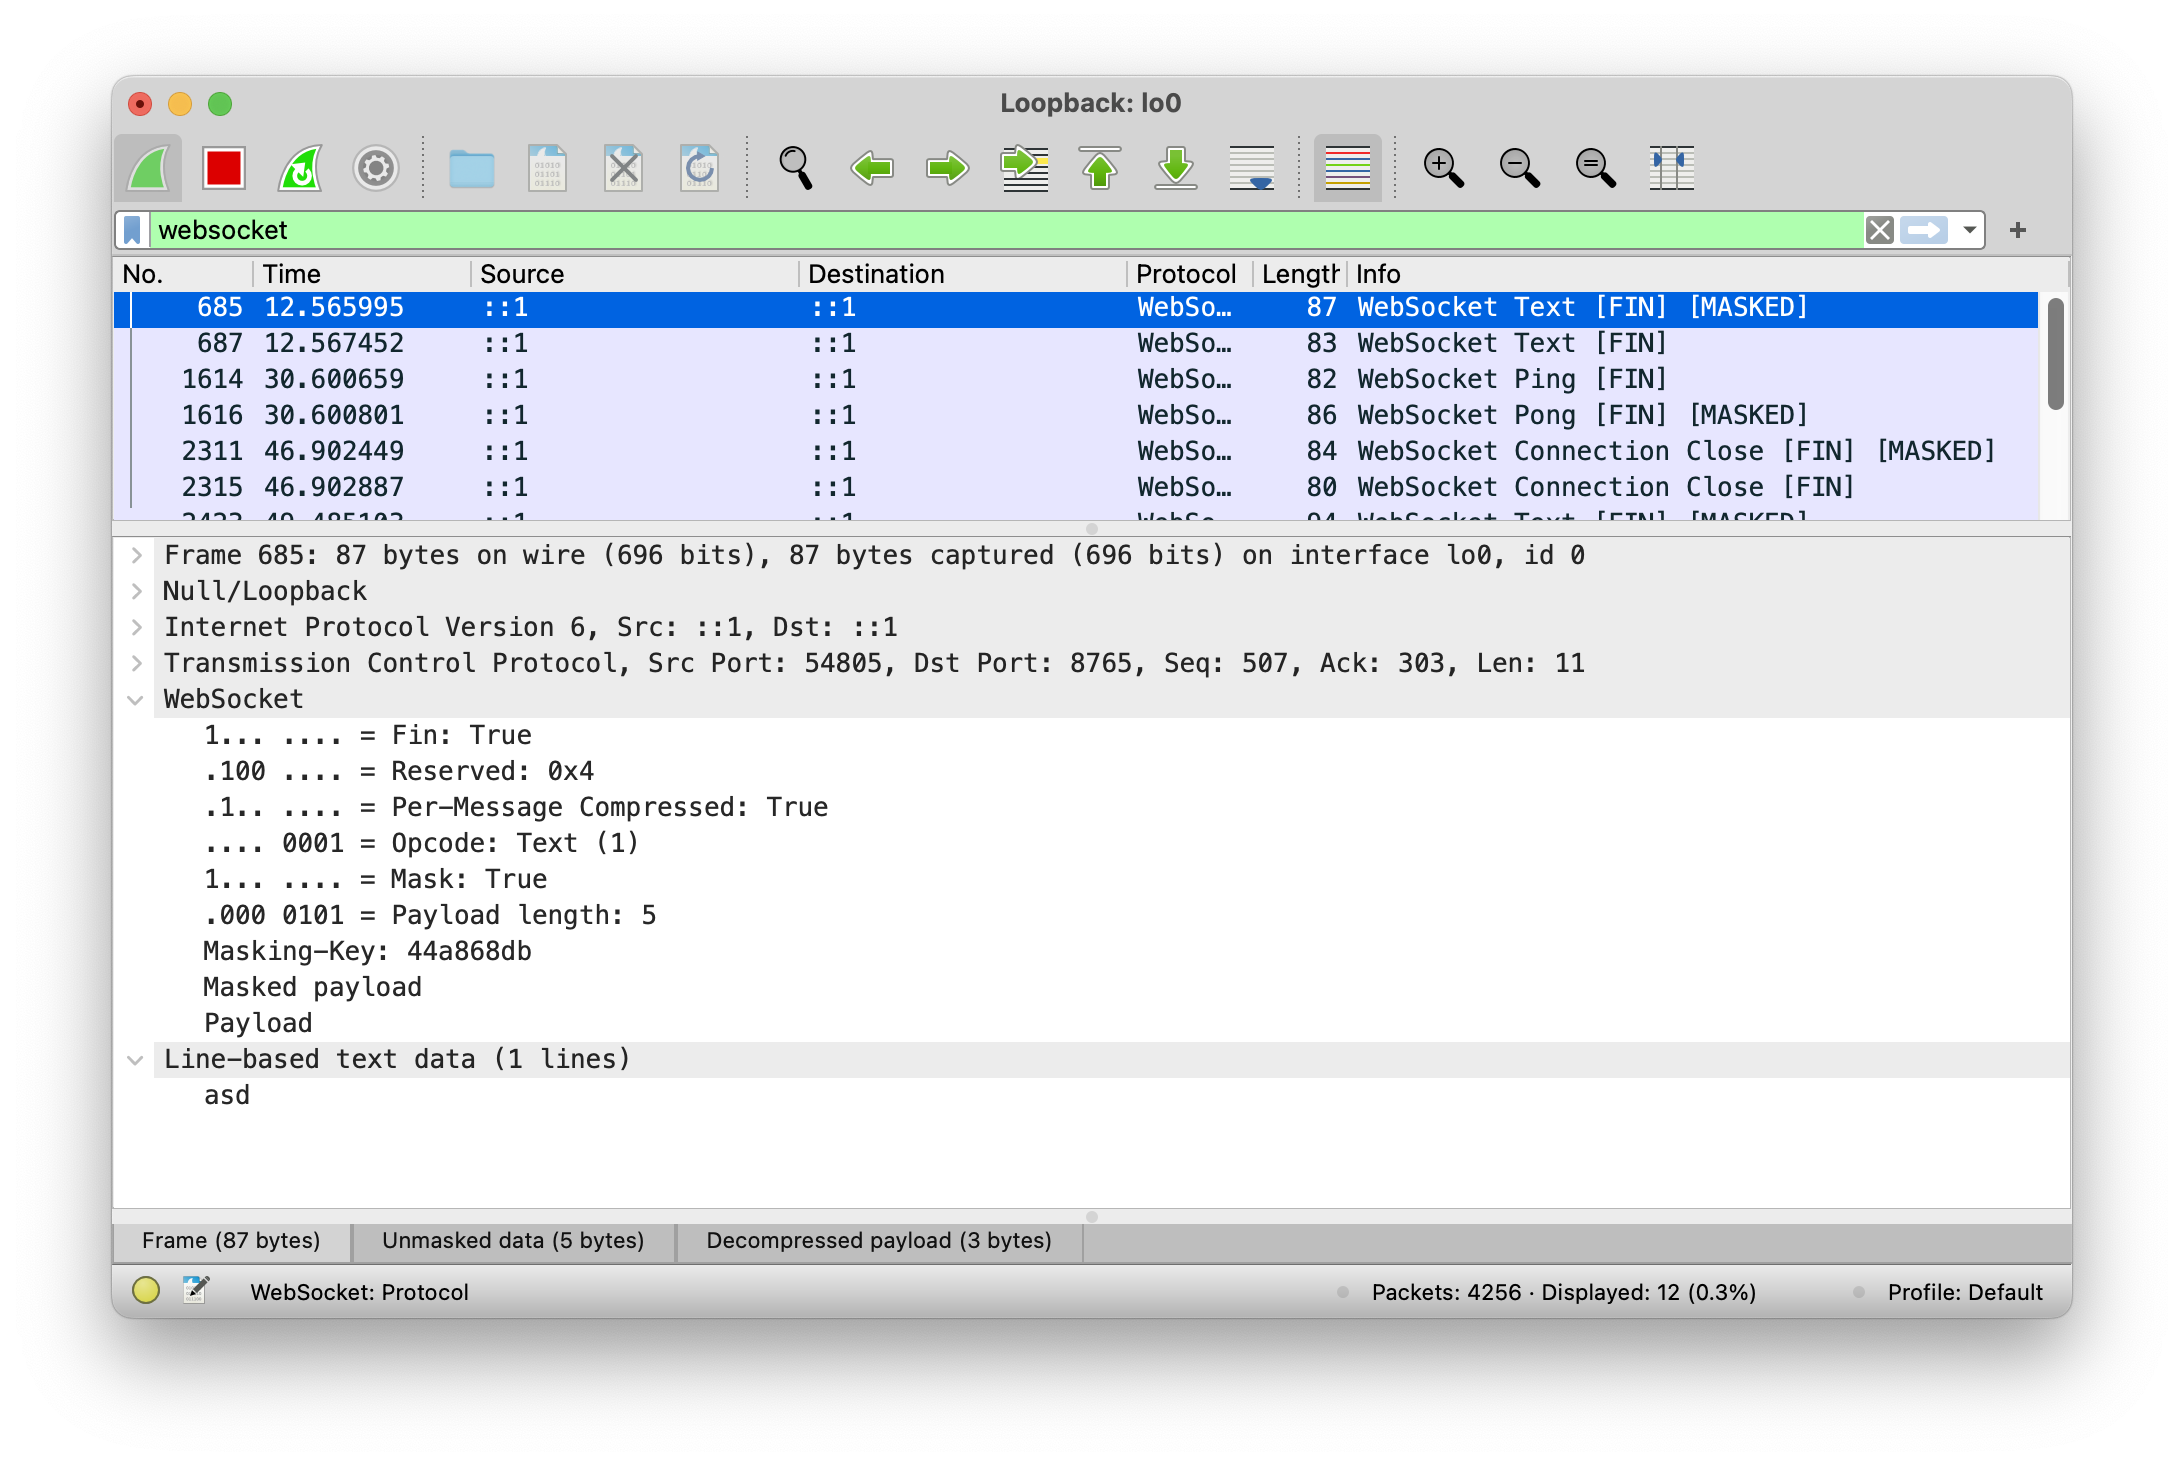
\includegraphics[height=14em]{res/ws}}

\section{Analysis}

\subsection{Design Diagram}
The biggest different between HTTP and WebSocket is that, HTTP is unidirectional while WebSocket is bidirectional and full-duplex.
When a client sends an HTTP request to the server, a TCP connection is open between the client and server, after getting the response, the TCP connection will be terminated, each HTTP request opens a separate TCP connection to the server. Here are two cons for the danmaku scenario: \ding{172} The server cannot send message to a client initiatively, since the server doesn't remember the IP address and the port number of the clients that need (subscribe?) the service. Under this situation, the client has to send requests to get the response initiatively and regularly. \ding{173} The polling mechanism can receive new danmakus, but not good enough. The latency may get even larger when the server needs to serve many clients that set the polling time interval larger. Also, the cost of performance of the server grows fast as the users are getting more and more. Now back to WebSocket, it easily solve the above two problems, yet the cost of keeping many connections between the server and each client may be appreciable.\\

\centerline{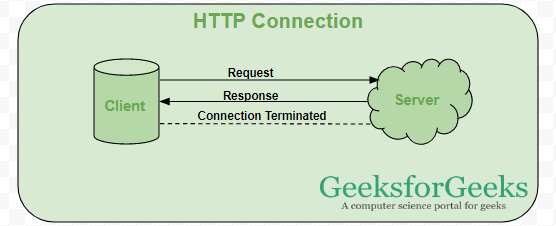
\includegraphics[width=0.45\textwidth]{res/httpi}\quad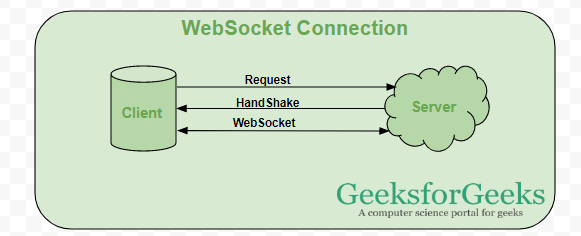
\includegraphics[width=0.45\textwidth]{res/wsi}}

\centerline{\scriptsize{src: www.geeksforgeeks.org/what-is-web-socket-and-how-it-is-different-from-the-http}}

\subsection{Network Traffic}
As we mentioned in the last section, the client using HTTP protocol has to send many request packages over the time, unfortunately, in the most of time there's no new message for the client, which means the most part of request packages sent by client (polling) contribute nothing for the service, but the resources are wasted.
\par Besides, since HTTP is stateless, the extra information must be carried in the header fields in a package, while the server under the WebSocket protocol remember the state of clients, and the packages are "lighter", in a word, the ratio of valid data, defined as data carrying info / (data + headers), of WebSocket is greater than the one of HTTP.

\subsection{Upgrade Efficiency}
Trivially, the latency of WebSocket is much less than the latency of HTTP. Since WebSocket can "broadcast" messages, or initiative send messages to client, the latency is the time to do operations on data and the time for packages to be transmit to the client, while the HTTP version's latency is "large or small" latency of polling (depends on the polling's frequency and the time of message is generated in a polling interval) and the time for doing operations and an even larger transmit time, since a new TCP connection needs to be established (handshaking) and the number of bits of headers are larger then the ws's headers.

\subsection{Comparison Summary}
We've notice that HTTP is stateless, in the scenarios that requires in-time data, that perform is awful, yet the server need not to keep the connections, which means it's more expandable (for the large amount of scenarios like browsing the net, watching videos, HTTP is fair enough and more fit to the public server that need to serve a large amount of users). If some serves need the message get just in time, WebSocket is much better than HTTP, such as the machines in labs, theating as servers, that may want to send message initiative to the endpoints acting as client, and the number of client won't be so large.


\end{document}
